
\documentclass[letterpaper]{article}
\usepackage[top=1.0in,bottom=1.0in,left=1.0in,right=1.0in]{geometry}
\usepackage{verbatim}
\usepackage{amssymb}
\usepackage{graphicx}
\usepackage{svg}
\usepackage{longtable}
\usepackage{amsfonts}
\usepackage{amsmath}
\usepackage{hyperref}
\usepackage{float}
\usepackage{caption}
\usepackage{xcolor}
\usepackage{adjustbox}
\usepackage{cleveref}

\bibliographystyle{elsarticle-num}
\def\thesection       {\arabic{section}}
\def\thesubsection     {\thesection.\alph{subsection}}

\author{Zoe Richter
        \\ \href{mailto:zrichte2@illinois.edu}{\texttt{zrichte2@illinois.edu}}
}
\title{20MWth Reactor Symmetry Sensitivity}
\begin{document}
\maketitle

Six Serpent2.0 models were run of a 20MWth htgr pebble-bed reactor with the following qualities:
\begin{itemize}
	\item $\frac{1}{6}$ core symmetry with periodic boundary condition
	\item 65 cm thickness graphite reflector on top and sides
	\item 50,000 neutrons and 100/50 active/inactive cycles in simulation
	\item 7 randomly distributed pebble compostions, each corresponding to a different level of burnup: fresh, 6 months, 12 months, 18 months, 24 months, 30 months, and 36 months
		\begin{itemize}
			\item Each pebble consists of a 2.5 cm radius homogenized fuel region surrounded by a 0.5 cm thick shell of graphite
		\end{itemize}
\end{itemize}

Each simulation was run for a different slice, as shown:

\begin{figure}[H]
\centerline{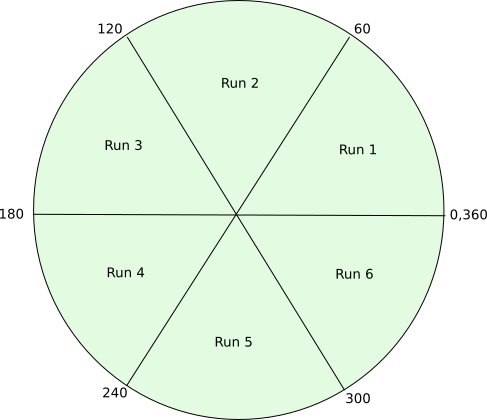
\includegraphics[width=8cm,keepaspectratio]{run-layout.png}}
\caption{Run Layout}
\label{layout}
\end{figure}

With all parameters except for which slice was used to represent the reactor remaining constant.
\\
The goal is to determine how $J^+$ at the outer reflector bound in the 20 MWth design compares to the "target" $J^+$ of the 200MWth design at the outer reflector bound.  To do this, the current given by the Serpent surface detector output, which is in $\frac{n}{s}$ and depends on the specific detector surface area, must be divided by the surface area of their respective detectors, like so:

\[ J^+_{i} [\frac{n}{cm^2s}] = \frac{J^+_{i} [\frac{n}{s}]}{S_{i} [cm^2]} \text{ where i is 20MWth or 200 MWth} \]

All simulations run for a 20MWth reactor design use the same detector size, shape and placement:  A cylinder of radius 164cm, and 328cm in height, centered at the origin.  These dimensions put the detector just inside the outermost boundary of the actual reflector (the detector was not put directly on the boundary to avoid the inaccuracies the boundary can cause.  The 200 MWth design also used a cylinder centered upon the origin, but of radius 215cm and height 1148cm.  The 200 MWth detector is similarly not on the exact outer bound of the reflector.

\begin{figure}[H]
\centerline{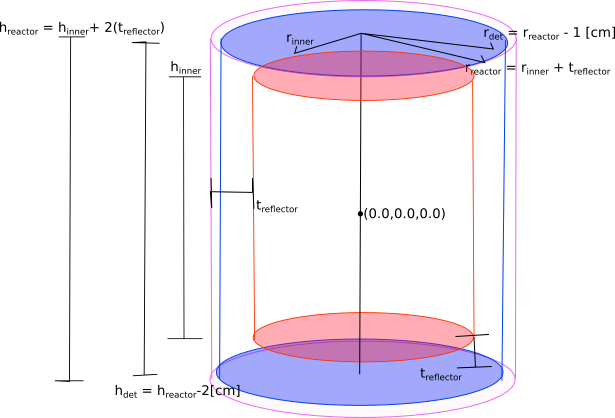
\includegraphics[width=8cm,keepaspectratio]{detector-layout.png}}
\caption{Diagram of Detector Surface (blue) in Reactor Model (pink,red)}
\label{top}
\end{figure}


The target outward current is 7.351e11, once the detector's surface area has been accounted for.

\begin{adjustbox}{max width=\textwidth}
\centering
 \begin{tabular}{|c | c | c | c | c|}
 	\hline \hline
 	Run & k & outer surface current $[\frac{n}{cm^2s}]$ & $J^+$ relative difference from full core & $J^+$ relative difference from 200MWth \\
 	\hline\hline
 	Run 1 & 1.03990 $\pm$ 0.00055 & 5.921e+11 $\pm$ 2.900e-09 & 0.637$\%$ & 19.449$\%$ decrease \\
 	Run 2 & 1.03979 $\pm$ 0.00050 & 5.884e+11 $\pm$ 2.781e-09 & 0.000$\%$ & 19.959$\%$ decrease \\
 	Run 3 & 1.04150 $\pm$ 0.00054 & 5.908e+11 $\pm$ 2.485e-09 & 0.402$\%$ & 19.637$\%$ decrease \\
 	Run 4 & 1.03927 $\pm$ 0.00057 & 5.910e+11 $\pm$ 2.900e-09 & 0.436$\%$ & 19.610$\%$ decrease \\
 	Run 5 & 1.04154 $\pm$ 0.00054 & 5.884e+11 $\pm$ 2.978e-09 & 0.000$\%$ & 19.959$\%$ decrease \\
 	Run 6 & 1.04047 $\pm$ 0.00050 & 5.888e+11 $\pm$ 2.840e-09 & 0.067$\%$ & 19.905$\%$ decrease \\
 	\hline


 \end{tabular}
\end{adjustbox}

Based on the table above, 75cm of graphite for the reflector should be sufficient to protect the RPV from fast neutron flux.  Additionally, the relative change between the results for a full core model and $\frac{1}{6}$ is small.
\\

The above analysis is for a sensitivity test with changing the "slice" of the reactor chosen to be the representative piece.  A similar analysis was done for a "scrambling" set of runs.  With the slice from Run 1 being the start, the pebble burnup locations were mixed up as follows: \\

\begin{center}
Original (Run 1):\\
Positions "0": Burnup 0\\
Positions "1": Burnup 1\\
Positions "2": Burnup 2\\
Positions "3": Burnup 3\\
Positions "4": Burnup 4\\
Positions "5": Burnup 5\\
Positions "6": Burnup 6\\
\end{center}
\begin{center}
Run 2: \\
Positions "0": Burnup 6\\
Positions "1": Burnup 0\\
Positions "2": Burnup 1\\
Positions "3": Burnup 2\\
Positions "4": Burnup 3\\
Positions "5": Burnup 4\\
Positions "6": Burnup 5\\
\end{center}
\begin{center}
Run 3:\\
Positions "0": Burnup 5\\
Positions "1": Burnup 6\\
Positions "2": Burnup 0\\
Positions "3": Burnup 1\\
Positions "4": Burnup 2\\
Positions "5": Burnup 3\\
Positions "6": Burnup 4\\
\end{center}
\begin{center}
Run 4:\\
Positions "0": Burnup 4\\
Positions "1": Burnup 5\\
Positions "2": Burnup 6\\
Positions "3": Burnup 0\\
Positions "4": Burnup 1\\
Positions "5": Burnup 2\\
Positions "6": Burnup 3\\
\end{center}
\begin{center}
Run 5:\\
Positions "0": Burnup 3\\
Positions "1": Burnup 4\\
Positions "2": Burnup 5\\
Positions "3": Burnup 6\\
Positions "4": Burnup 0\\
Positions "5": Burnup 1\\
Positions "6": Burnup 2\\
\end{center}
\begin{center}
Run 6:\\
Positions "0": Burnup 2\\
Positions "1": Burnup 3\\
Positions "2": Burnup 4\\
Positions "3": Burnup 5\\
Positions "4": Burnup 6\\
Positions "5": Burnup 0\\
Positions "6": Burnup 1\\
\end{center}
\begin{center}
Run 7:\\
Positions "0": Burnup 1\\
Positions "1": Burnup 2\\
Positions "2": Burnup 3\\
Positions "3": Burnup 4\\
Positions "4": Burnup 5\\
Positions "5": Burnup 6\\
Positions "6": Burnup 0\\
\end{center}

\begin{adjustbox}{max width=\textwidth}
\centering
 \begin{tabular}{|c | c | c | c | c|}
 	\hline \hline
 	Run & k & outer surface current $[\frac{n}{cm^2s}]$ & $J^+$ relative difference from full core & $J^+$ relative difference from 200MWth \\
 	\hline\hline
 	Run 1 & 1.03990 $\pm$ 0.00055 & 5.921e+11 $\pm$ 2.900e-09 & 0.637$\%$ & 19.449$\%$ decrease \\
 	Run 2 & 1.04067 $\pm$ 0.00050 & 5.908e+11 $\pm$ 3.057e-09 & 0.402$\%$ & 19.637$\%$ decrease \\
 	Run 3 & 1.04133 $\pm$ 0.00055 & 5.888e+11 $\pm$ 2.584e-09 & 0.067$\%$ & 19.905$\%$ decrease \\
 	Run 4 & 1.04206 $\pm$ 0.00058 & 5.906e+11 $\pm$ 2.840e-09 & 0.369$\%$ & 19.664$\%$ decrease \\
 	Run 5 & 1.03850 $\pm$ 0.00060 & 5.929e+11 $\pm$ 2.742e-09 & 0.771$\%$ & 19.342$\%$ decrease \\
 	Run 6 & 1.03874 $\pm$ 0.00052 & 5.939e+11 $\pm$ 2.604e-09 & 0.939$\%$ & 19.207$\%$ decrease \\
 	Run 6 & 1.03746 $\pm$ 0.00058 & 5.949e+11 $\pm$ 2.623e-09 & 1.106$\%$ & 19.073$\%$ decrease \\
 	\hline


 \end{tabular}
\end{adjustbox}

\end{document}